\section{Clustering}
We now run and compare some clustering algorithm in order to find some structures among the data. First we start with a basic \emph{K-Means} followed with some \emph{Hierarchical clustering techniques} and \emph{DBSCAN}. 
\subsection{Preprocessing}

\begin{wrapfigure}[10]{r}{0.5\textwidth}
\vspace{-13mm}
\centering
\captionsetup{justification=centering}
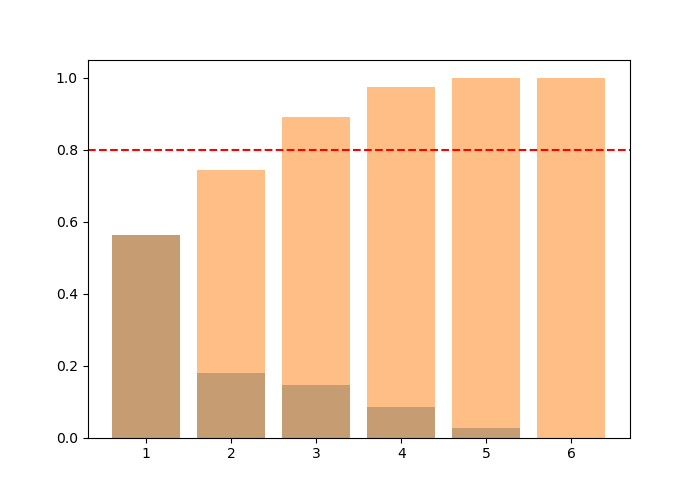
\includegraphics[width=.5\textwidth]{img/clust_1/pca.png}
\caption{Explained variance ratio}
\label{fig:pca_img}
\end{wrapfigure}

The data matrix was first standardized and then the two principal components were extracted. The choice was between two and tree principal component since they retain respectively $\sim$0.75 and $\sim$0.85 of the variance of the data.

We selected the two principal components because it performed better on K-Means and, in this way, we could also have a visual inspection.

\subsection{K-Means}
The algorithm run for $K$ ranging from 2 to 10 clusters. For each iteration the SSE and the average silhouette value were computed.

\begin{figure}[h!]
     \captionsetup{justification=centering}		
     \centering
     \begin{subfigure}{0.32\textwidth}
         \centering
         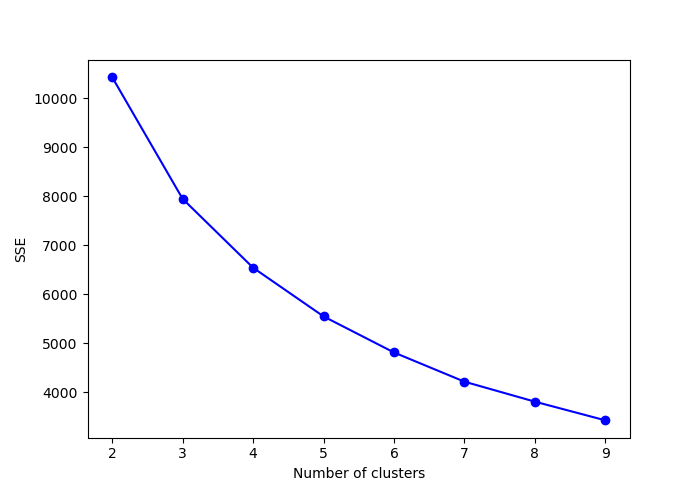
\includegraphics[width=\textwidth]{img/clust_1/sse.png}
         \caption{SSE}
         \label{fig:sse_img}
     \end{subfigure}
     \begin{subfigure}{0.32\textwidth}
         \centering
         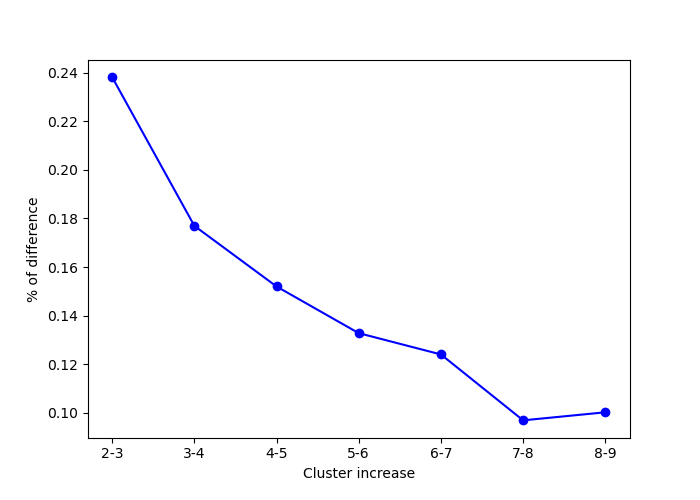
\includegraphics[width=\textwidth]{img/clust_1/perc.png}
         \caption{\% of decrease in SSE}
         \label{fig:pdiff_img}
     \end{subfigure}
     \begin{subfigure}{0.32\textwidth}
         \centering
         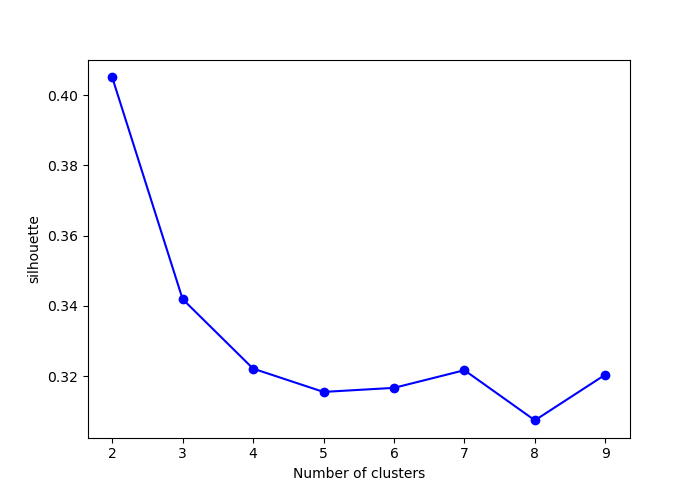
\includegraphics[width=\textwidth]{img/clust_1/sil.png}
         \caption{Average silhouette}
         \label{fig:sil_img}
     \end{subfigure}
     \caption{\emph{K-Means} metrics}
    \label{fig:km_metrics}
\end{figure}

By looking at the plots in Figure \ref{fig:km_metrics}, we can see that there isn't a prominent \emph{elbow shape}, so we needed the analysis of more metrics to get the optimal number of clusters. At first, we saw that, for $K$ moving from 2 to 3, the difference of the SSE in percentage was quite high ($\sim$0.24), while for all the other values the difference was below 0.2. By inspecting the silhouette score, it is possible to see that it has its maximum for $K = 2$, followed by $K = 3$. In conclusion, we opted for 3 clusters, to get a trade off between high silhouette and low SSE.

\begin{wrapfigure}[13]{l}{.5\textwidth}
    \vspace{-2mm}
    \centering
    \captionsetup{justification=centering}
    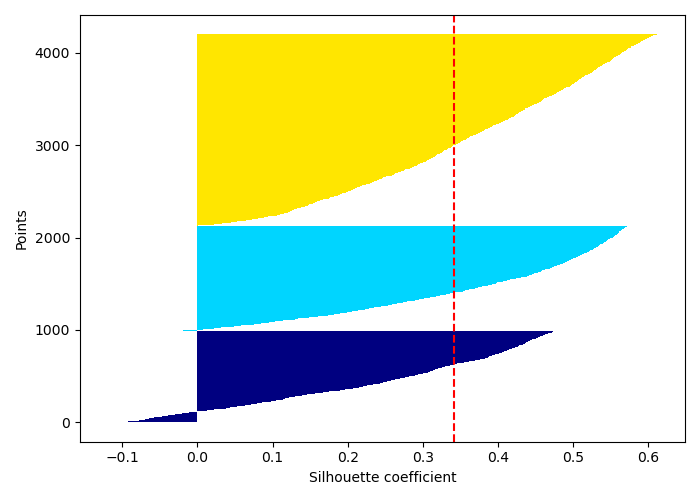
\includegraphics[width=.5\textwidth]{img/clust_1/sil_tot.png}
    \caption{Silhouette score\\ for each data point}
    \label{fig:silhouette}
\end{wrapfigure}

The resulting clusters have a comparable number of points. In particular \emph{Cluster 0} has \textbf{990} points, \emph{Cluster 1} \textbf{1137} and \emph{Cluster 2} \textbf{2072}.\\
In Figure \ref{fig:silhouette}, we can see the plot of the Silhouette score, where each different color represents a different cluster, and the dotted red line is the average silhouette score. 
We see that a small fraction of points in \emph{Cluster 1} and \emph{Cluster 0} have a negative value but overall the Silhouette suggests a good clustering.

\begin{figure}[h!]
    \centering
    \captionsetup{justification=centering}
    \begin{subfigure}{0.32\textwidth}
        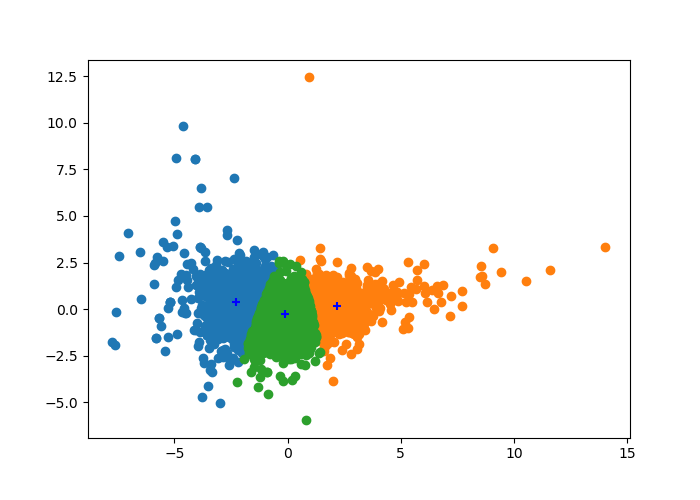
\includegraphics[width=\textwidth]{img/clust_1/km_clusters.png}
        \caption{Clustering result}
        \label{fig:skmclust}
    \end{subfigure}
    \begin{subfigure}{0.32\textwidth}
        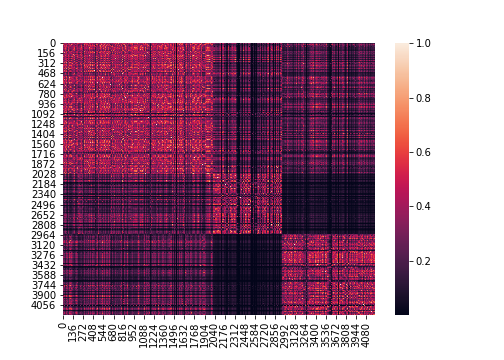
\includegraphics[width=\textwidth]{img/clust_1/sim_heatmap.png}
        \caption{Similarity heatmap}
        \label{fig:sim_heatmap}
    \end{subfigure}
    \begin{subfigure}{0.32\textwidth}
        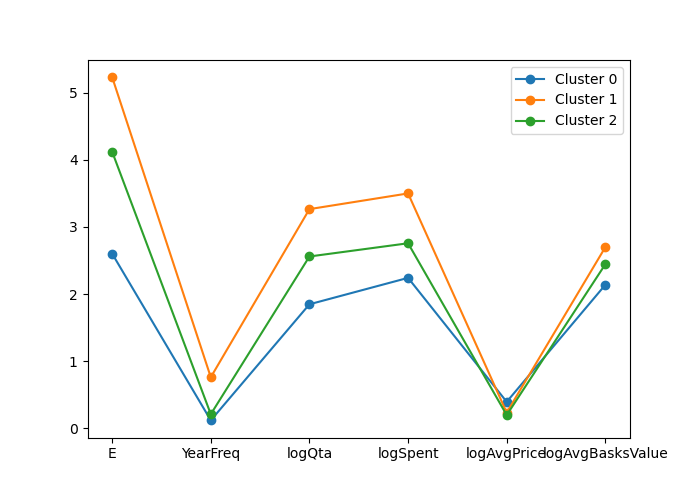
\includegraphics[width=\textwidth]{img/clust_1/cluster_avg.png}
	\caption{Average values\\ per cluster}
        \label{fig:km_avg}
    \end{subfigure}
\end{figure}

\begin{comment}
The plot shows the average values for each attribute divided by the clusters. In particular is possible to see that \emph{Cluster 0} contains the most frequent and spending customers, followed by \emph{Cluster 2} and \emph{Cluster 1}
\end{comment}

In Figure \ref{fig:skmclust}, we can appreciate the results of the algorithm, where we can see that the clusters are well separated from one another.\\
The similarity matrix (Figure \ref{fig:sim_heatmap}) shows the affinity of elements inside a cluster; we can see that the results are pretty good, and in particular \emph{Cluster 2} contains points really similar to each other.\\
Instead, the plot in Figure \ref{fig:km_avg} shows the average values for each attribute divided by the clusters. In particular, it is possible to see that \emph{Cluster 0} contains the most frequent and spending customers, followed by \emph{Cluster 2} and \emph{Cluster 1}.

\begin{comment}
\begin{figure}
    \captionsetup{justification=centering}
    \centering
    \begin{subfigure}{0.49\textwidth}
        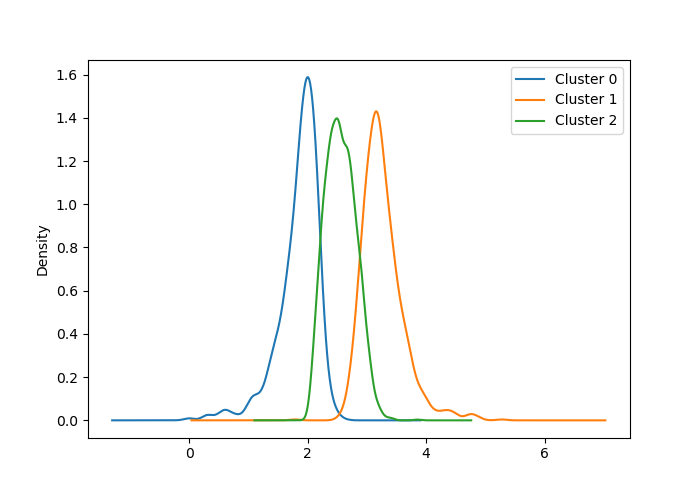
\includegraphics[width=.7\textwidth]{img/clust_1/logqta_km.png}
        \caption{Distributions of \emph{logQta}}
        \label{fig:logqta}
    \end{subfigure}
    \begin{subfigure}{0.49\textwidth}
        \centering
        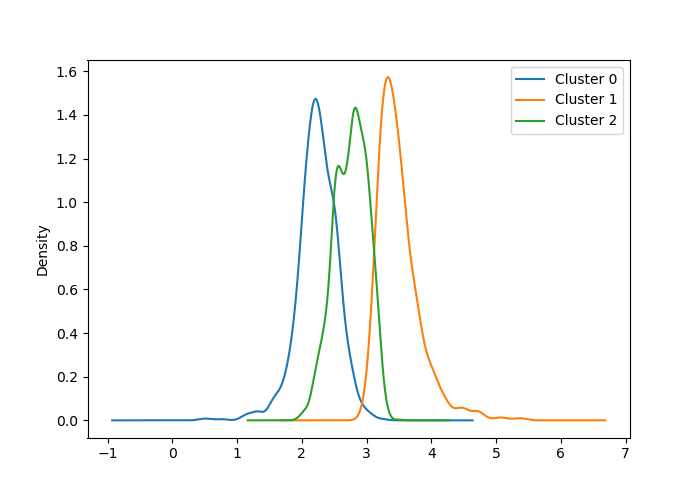
\includegraphics[width=.7\textwidth]{img/clust_1/logspent_km.png}
        \caption{Distribution of \emph{logSpent}}
        \label{fig:logspent}
    \end{subfigure}
        \begin{subfigure}{0.49\textwidth}
        \centering
        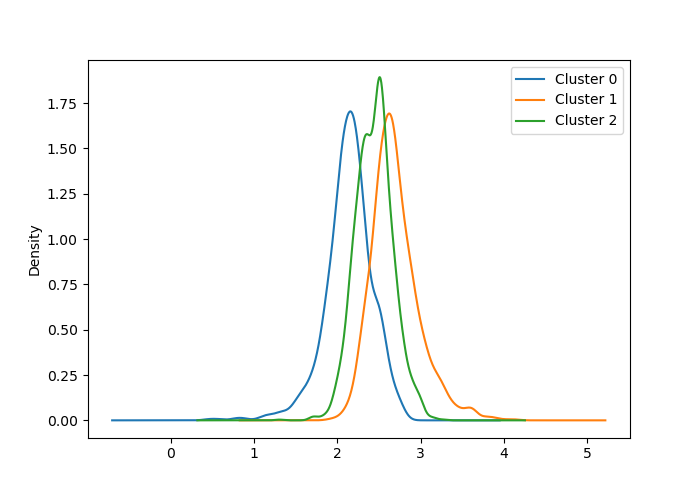
\includegraphics[width=.7\textwidth]{img/clust_1/logavgbv_km.png}
        \caption{Distribution of \emph{logAvgBasksValue}}
        \label{fig:logavgbv}
    \end{subfigure}
        \begin{subfigure}{0.49\textwidth}
        \centering
        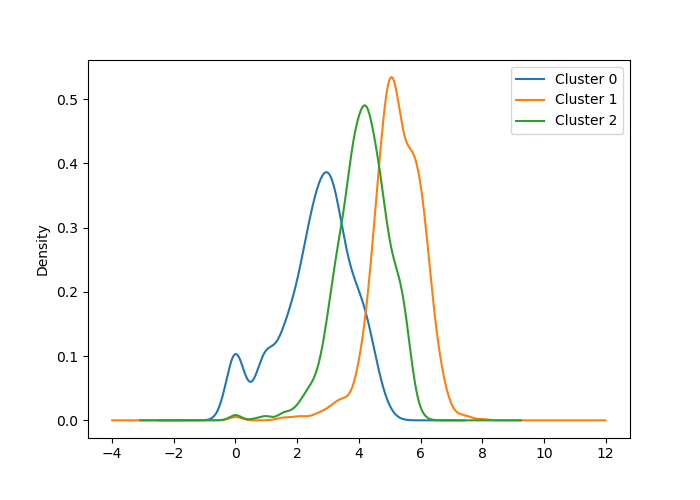
\includegraphics[width=.7\textwidth]{img/clust_1/tp_entr_km.png}
        \caption{Distribution of \emph{TPEntr}}
        \label{fig:tpentr}
    \end{subfigure}
    \caption{Distribution of some attribute based partitioned with respect the clusters}
\end{figure}
\end{comment}

\subsection{Hierarchical clustering}
We used different kinds of algorithm: \emph{Complete Link}, \emph{Single Link}, \emph{Ward} and \emph{Centroid}. The CPCC coefficient are respectively 0.51, 0.62, 0.44 and 0.74 meaning that the best results are obtained with \emph{Single Link} and \emph{Centroid}. By looking at the dendograms in Figure \ref{fig:dendograms}, if we cut the tree by selecting two clusters, we can see that the vast majority of the data falls into a single cluster, leaving the last merge between a large cluster and a small one, in some cases even a singleton. The most balanced result is obtained with the \emph{Ward} method, even though it has the lowest CPCC.

\begin{figure}
    \centering
    \begin{subfigure}{0.49\textwidth}
        \centering
        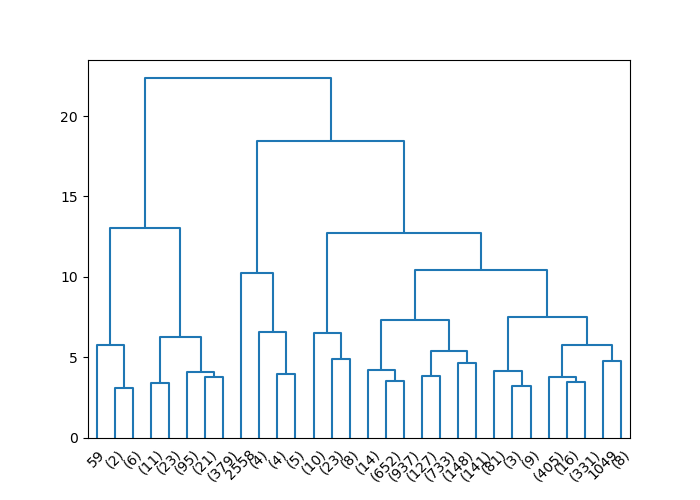
\includegraphics[width=0.7\textwidth]{img/clust_1/c_link.png}
        \caption{\emph{Complete Link}}
        \label{fig:clink_img}
    \end{subfigure}
    \begin{subfigure}{0.49\textwidth}
        \centering
        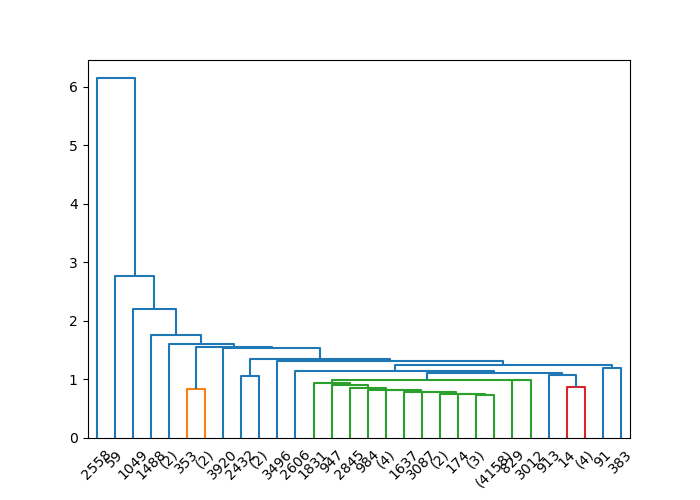
\includegraphics[width=0.7\textwidth]{img/clust_1/s_link.png}
        \caption{\emph{Single Link}}
        \label{fig:slink_img}
    \end{subfigure}
    \begin{subfigure}{0.49\textwidth}
        \centering
        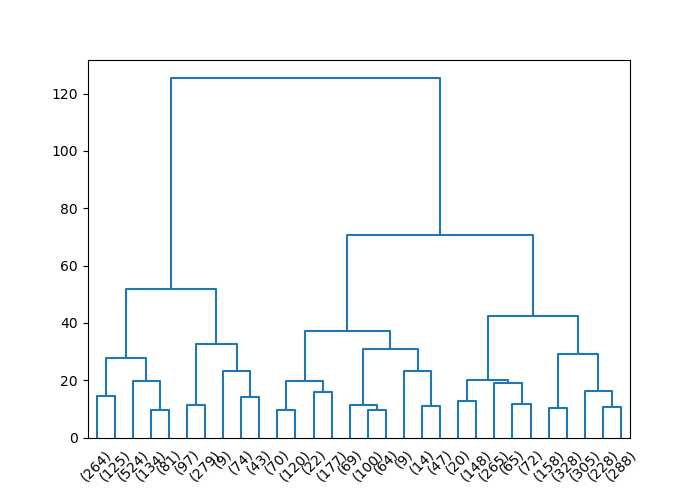
\includegraphics[width=0.7\textwidth]{img/clust_1/ward.png}
        \caption{\emph{Ward}}
        \label{fig:ward_img}
    \end{subfigure}
    \begin{subfigure}{0.49\textwidth}
         \centering
         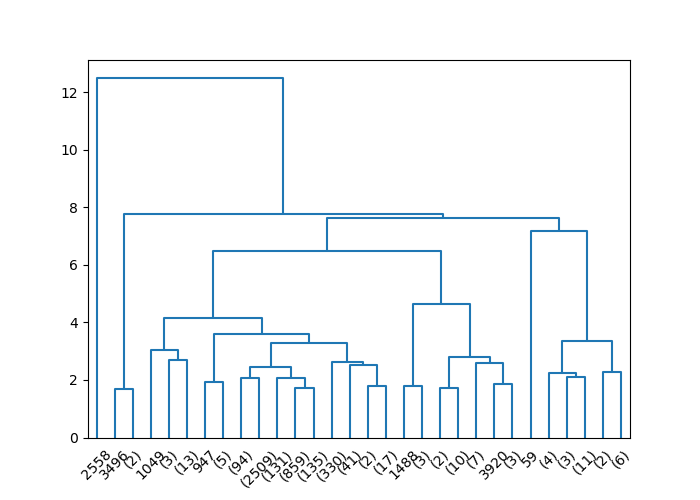
\includegraphics[width=0.7\textwidth]{img/clust_1/centroid.png}
         \caption{\emph{Centroids}}
         \label{fig:centr_img}
     \end{subfigure}
     \caption{}
    \label{fig:dendograms}
\end{figure}

\subsection{DBSCAN}

\begin{figure}[h!]
	\captionsetup{justification=centering}
	\centering
	\begin{subfigure}{0.49\textwidth}
		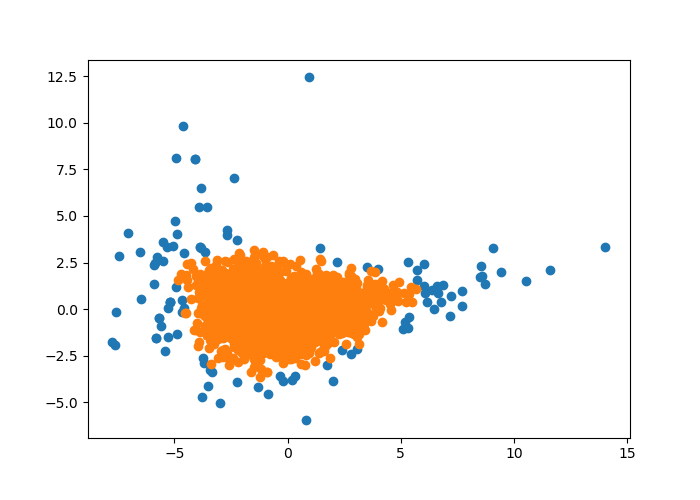
\includegraphics[width=.65\textwidth]{img/clust_1/dbscan.png}
		\centering
		\label{fig:dbscan_good}
	\end{subfigure}
	\begin{subfigure}{0.49\textwidth}
		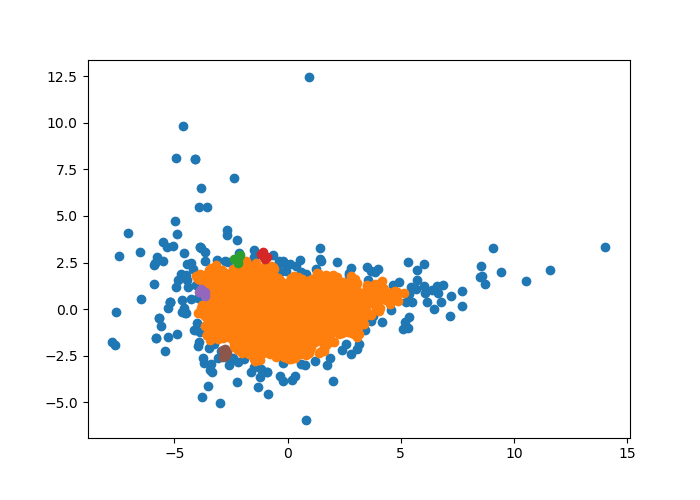
\includegraphics[width=.65\textwidth]{img/clust_1/dbscan_bad.png}
		\centering
		\label{fig:dbscan_bad}
	\end{subfigure}
	\caption{Results of DBSCAN}
	\label{fig:dbscan}
\end{figure}

We explored different combination of \emph{eps} and \emph{MinPts}; for a given value of \emph{MinPts}, we selected \emph{eps} by checking the \emph{KNN} distance, with $K$ equal to \emph{MinPts}.\\
Some results are plotted in Figure \ref{fig:dbscan}. In the first case, with \emph{eps}$= 0.6$ and \emph{MinPts}$=8$, we have a large and cluster surrounded by noise points; in the second one, with \emph{eps}$=0.3$ and \emph{MinPts}$=5$, we still have a large cluster, but also a lot of other clusters, really small if compared to the central one.\\
For that, we think that the dataset is not suitable for this kind of algorithm.
